% \begin{frame}{Alternate Efficiency Definition}
%     \begin{itemize}
%         \item Remove acceptance based on fiducial cuts at truth level
%         \item Define Efficiency as the fraction of events with exactly 2 reconstructed longTracks divided by the total number of events. 
%         \[ \text{Efficiency} = \frac{\text{NEvents}({= 2 \text{longTracks}}\ | \ \text{Fiducial})}{\text{NEvents}(\geq0{\text{longTracks}}\ | \ \text{Fiducial})} \]
%     \end{itemize}
% \end{frame}

% \begin{frame}{2 Track Efficiency as a function of DeltaR}
%     \begin{figure}
%         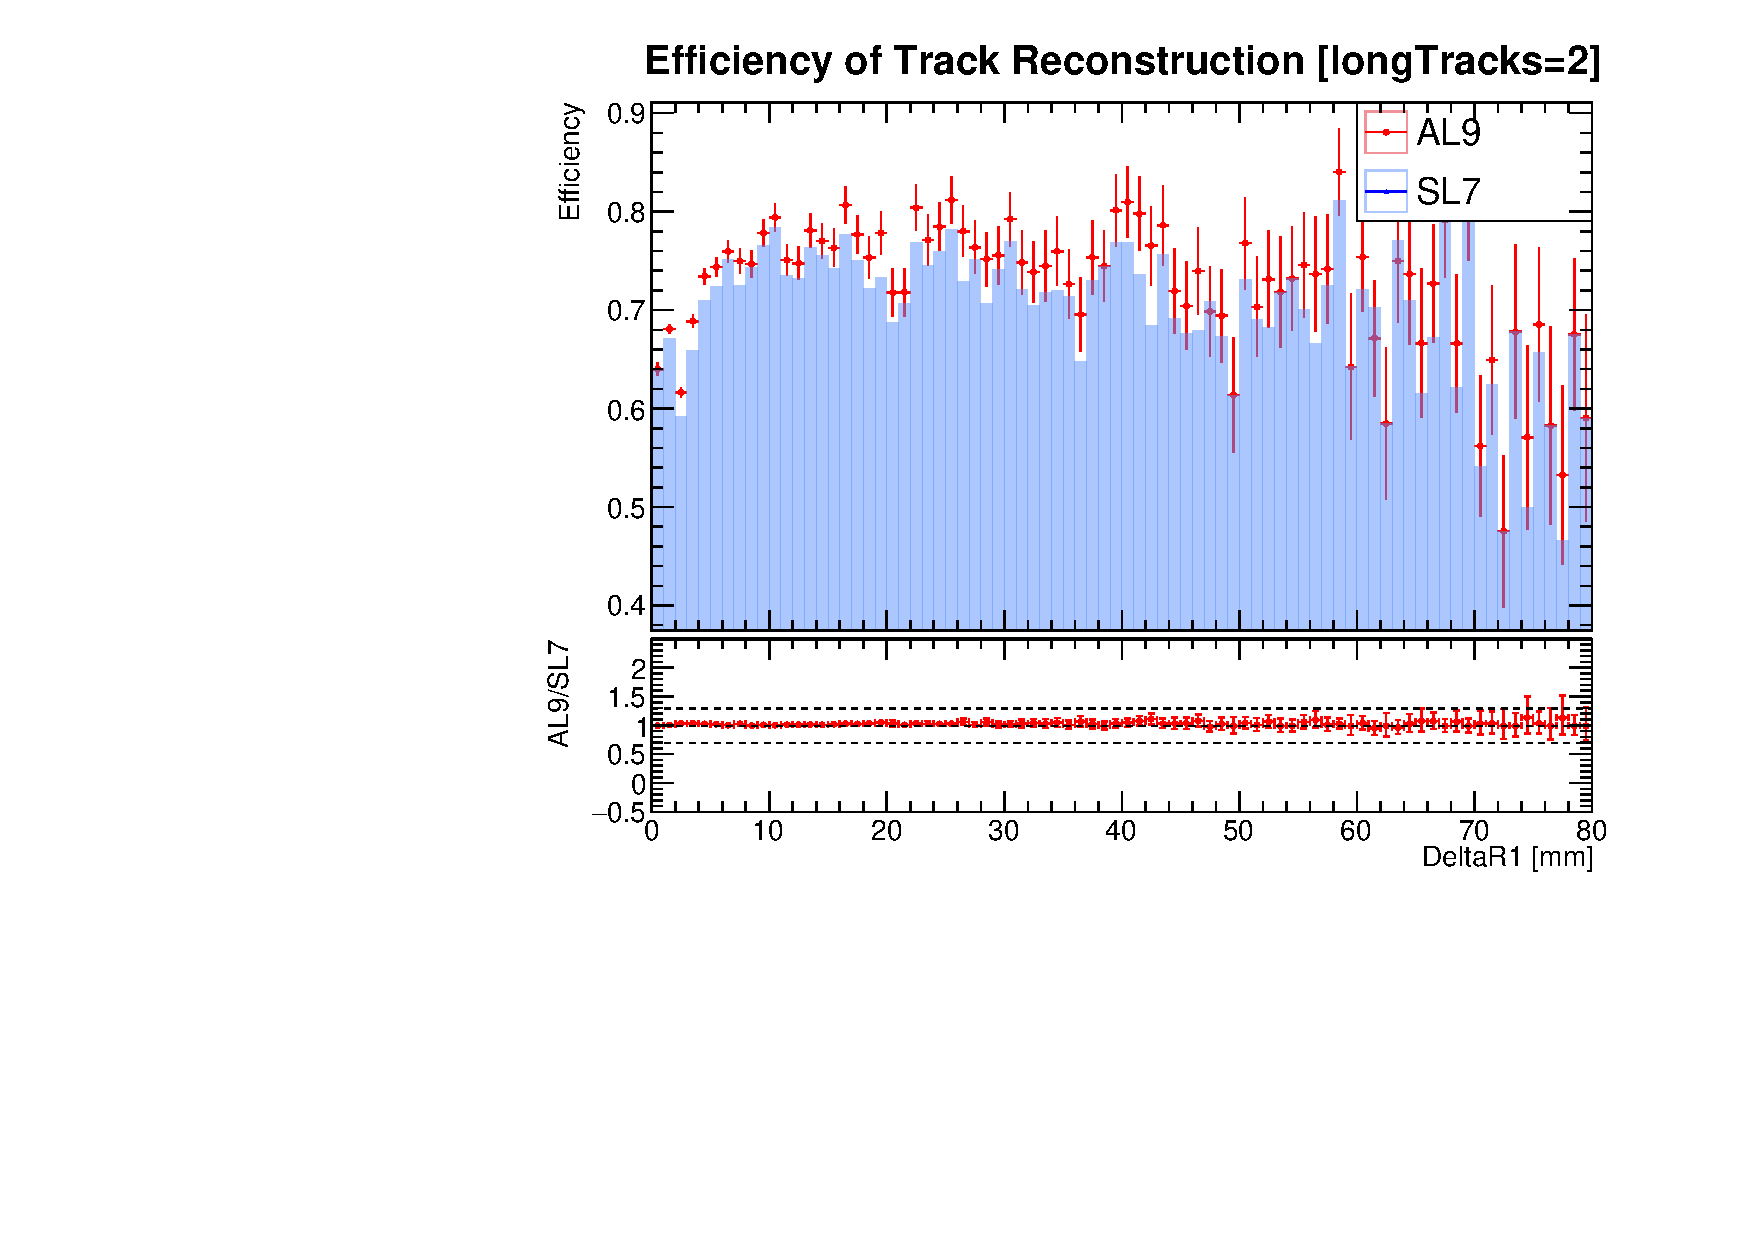
\includegraphics[width=\linewidth]{./output/Effi_eq2_DeltaR1.pdf}
%     \end{figure}
% \end{frame}

% \begin{frame}{2 Track Efficiency as a function of DeltaX0 [SKIP]}
%     \begin{figure}
%         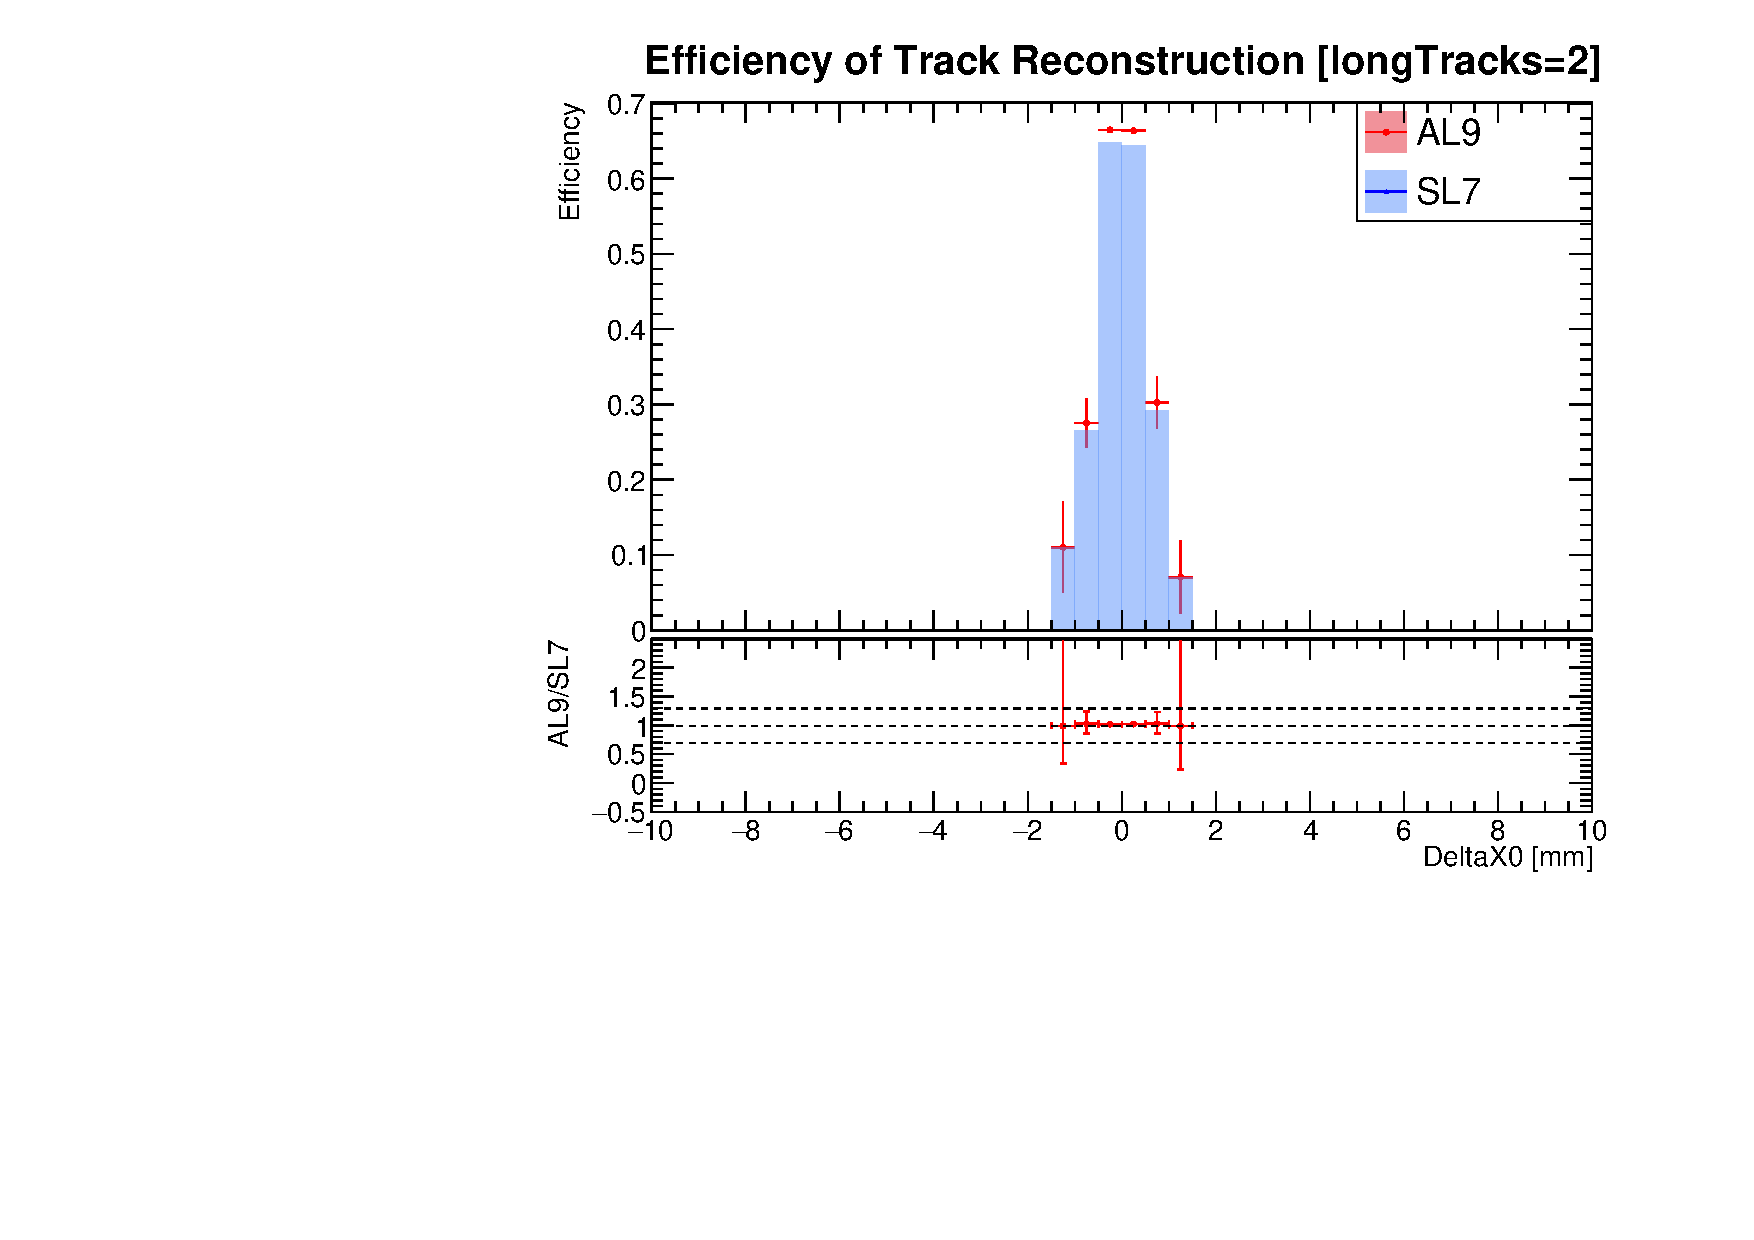
\includegraphics[width=\linewidth]{./output/Effi_eq2_DeltaX0.pdf}
%     \end{figure}
% \end{frame}
% \begin{frame}{2 Track Efficiency as a function of DeltaY0 [SKIP]}
%     \begin{figure}
%         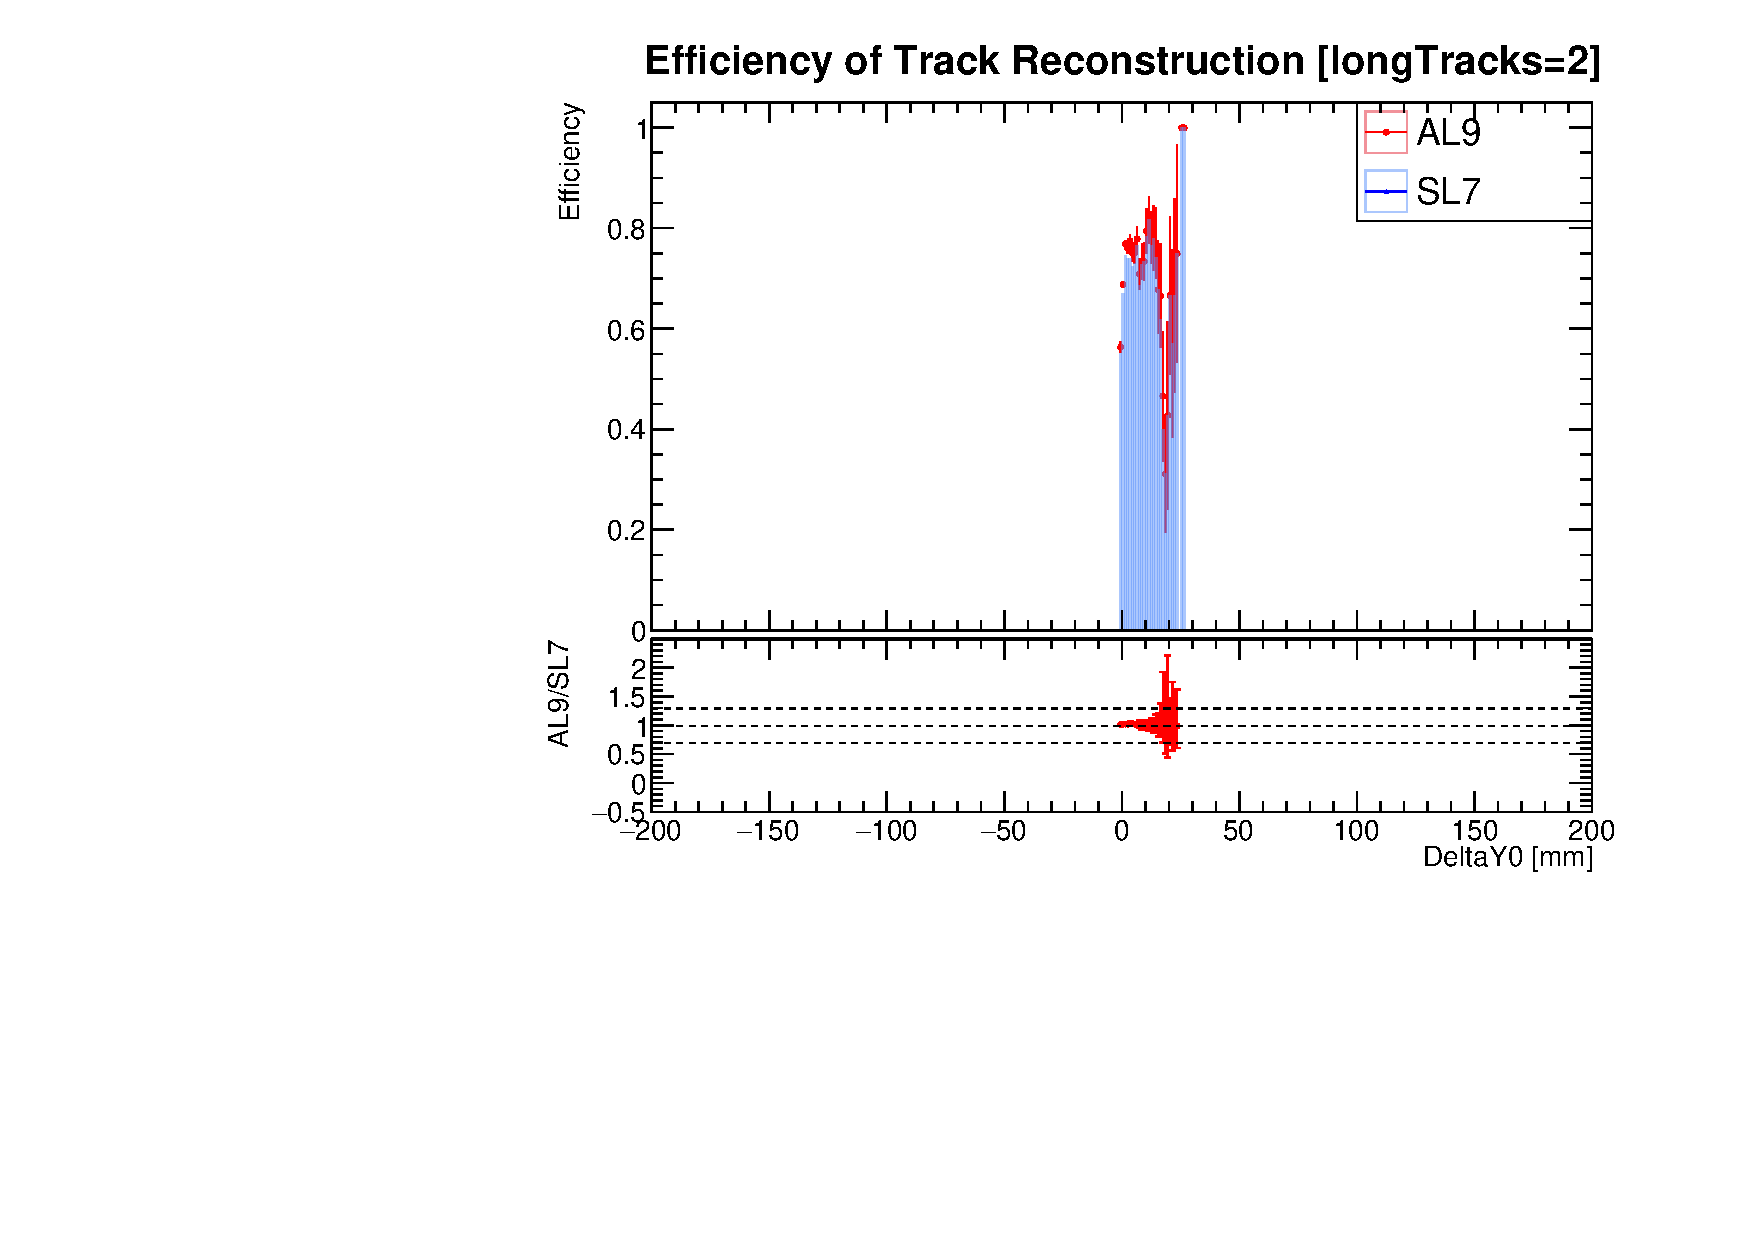
\includegraphics[width=\linewidth]{./output/Effi_eq2_DeltaY0.pdf}
%     \end{figure}
% \end{frame}

% \begin{frame}{2 Track Efficiency as a function of Theta1}
%     \begin{figure}
%         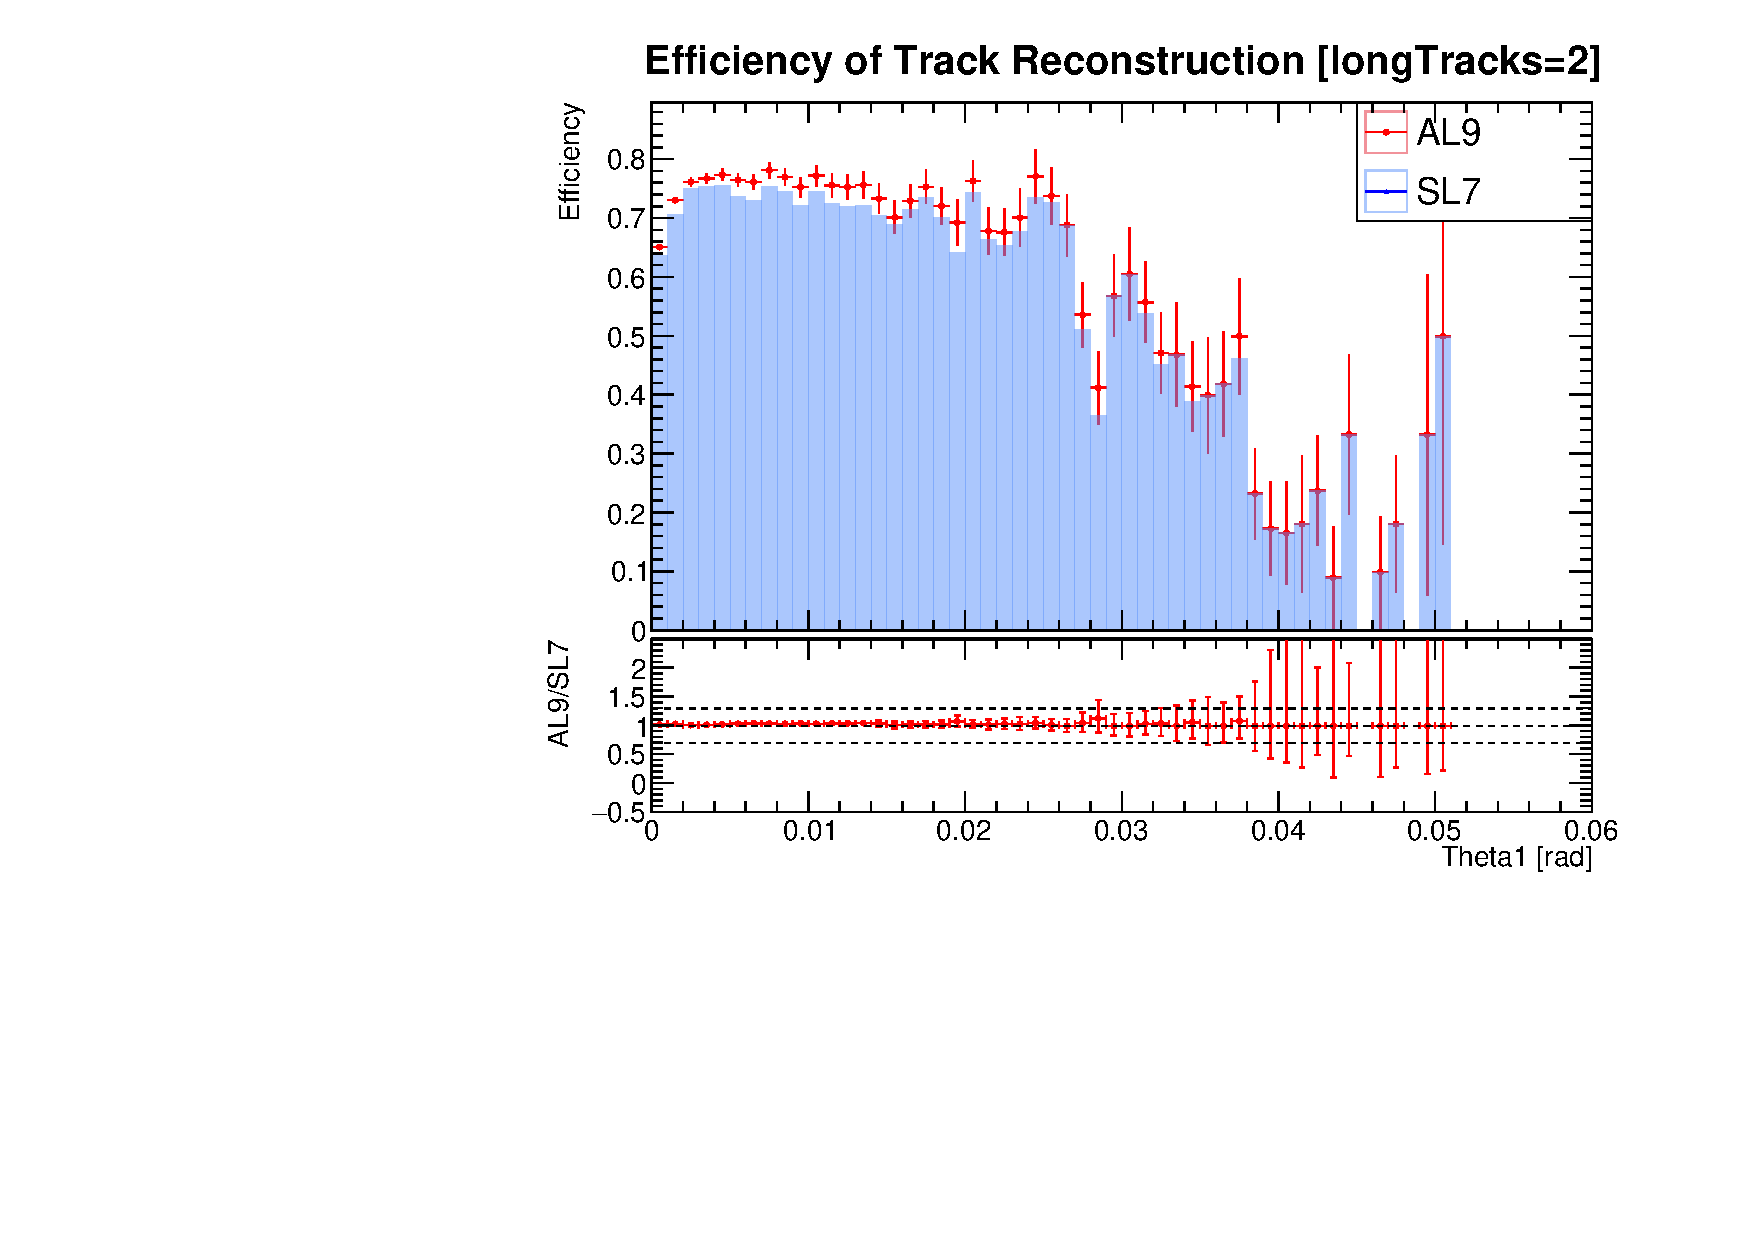
\includegraphics[width=\linewidth]{./output/Effi_eq2_Theta1.pdf}
%     \end{figure}
% \end{frame}
% \begin{frame}{2 Track Efficiency as a function of DeltaRP}
%     \begin{figure}
%         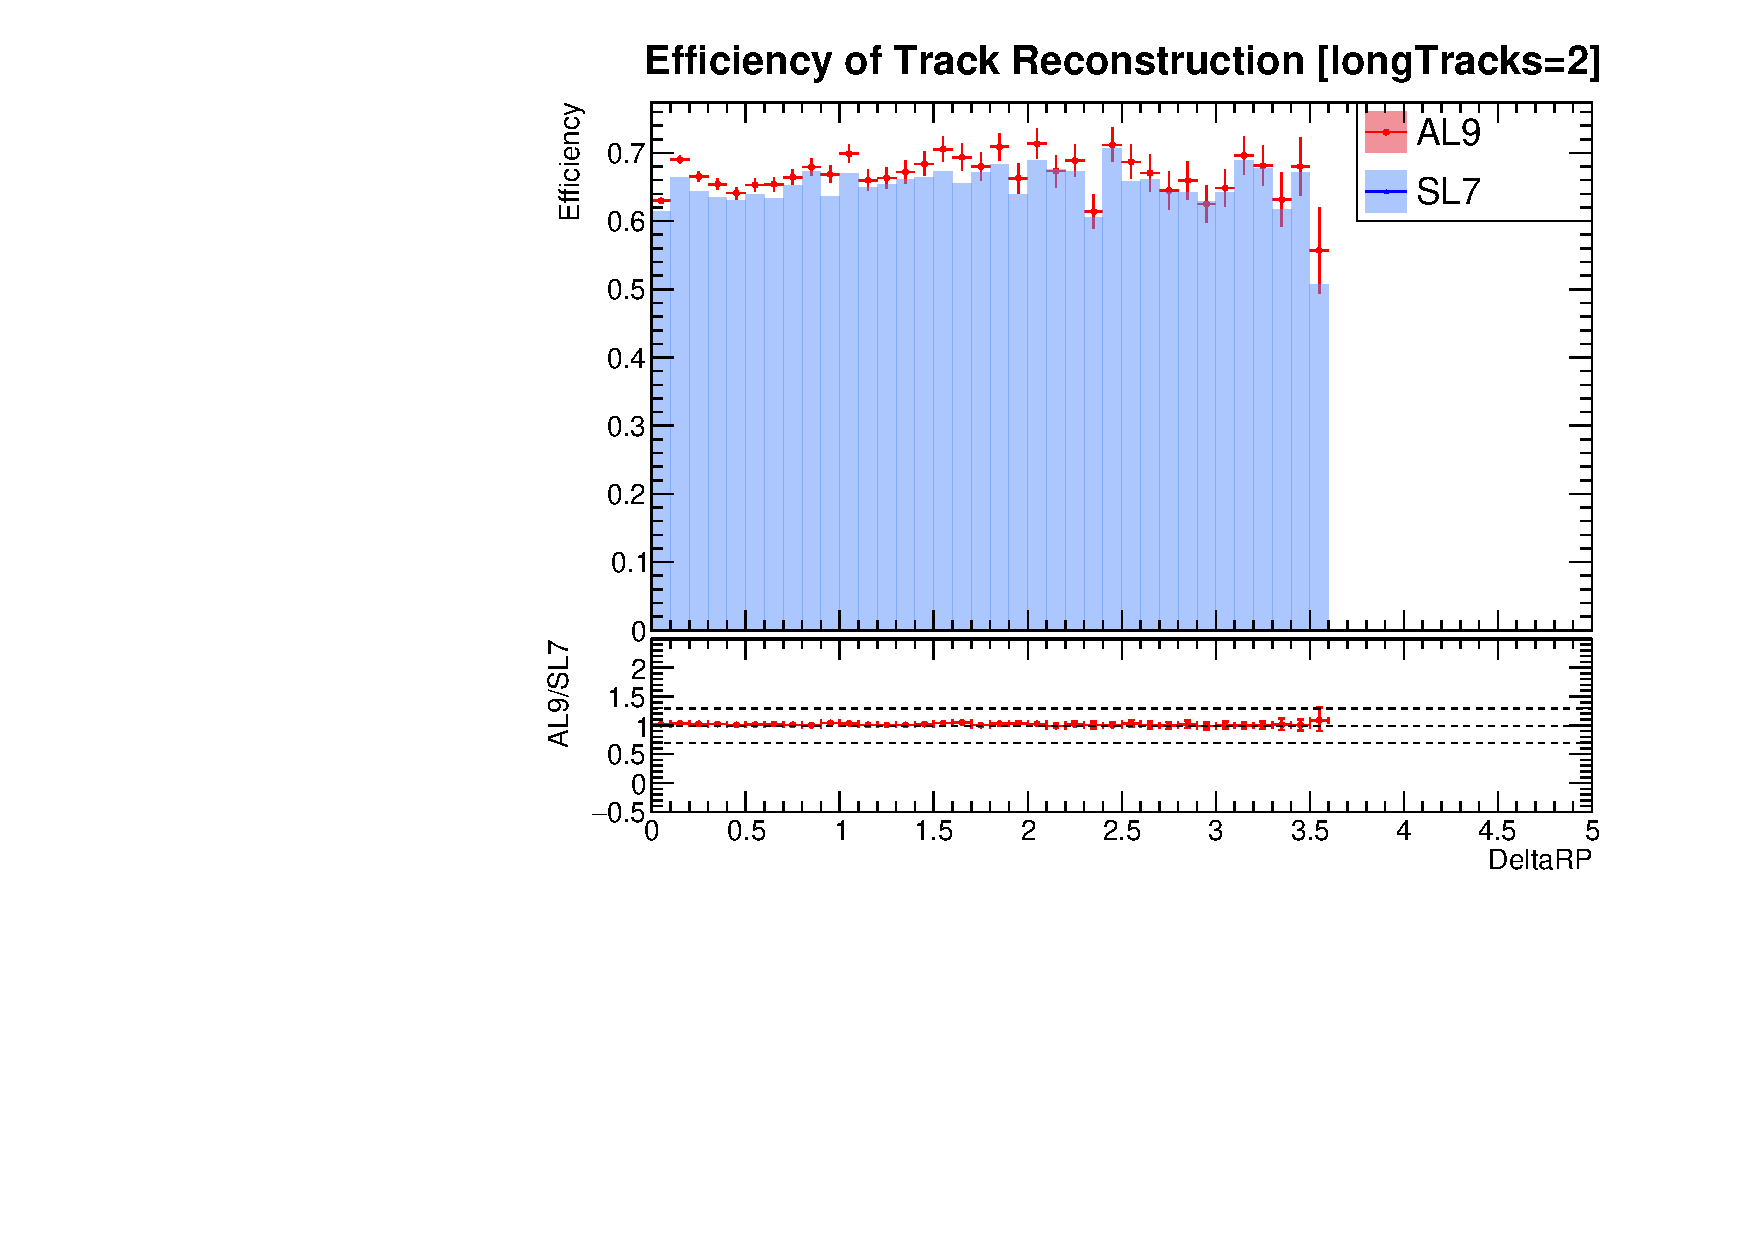
\includegraphics[width=\linewidth]{./output/Effi_eq2_DeltaRP.pdf}
%     \end{figure}
% \end{frame}